\documentclass{article}
\usepackage[utf8]{inputenc}
\usepackage{graphicx}
\usepackage{amsmath} 

\title{Computer graphics - cylindres}
\author{samuel.chassot }
\date{February 2019}

\usepackage{natbib}
\usepackage{graphicx}

\begin{document}

\maketitle

\section{Infinite length cylinder}
Let us take a cylinder with $c + v_a*k$ as axis and $r$ as radius. For a point of the space $q = (x,y,z)$, it is on the cylinder iif the distance between the axis and the point (red $r$ on the sketch) is equal to $r$.

Here is a sketch of the situation:
\begin{figure}[h]
\centering
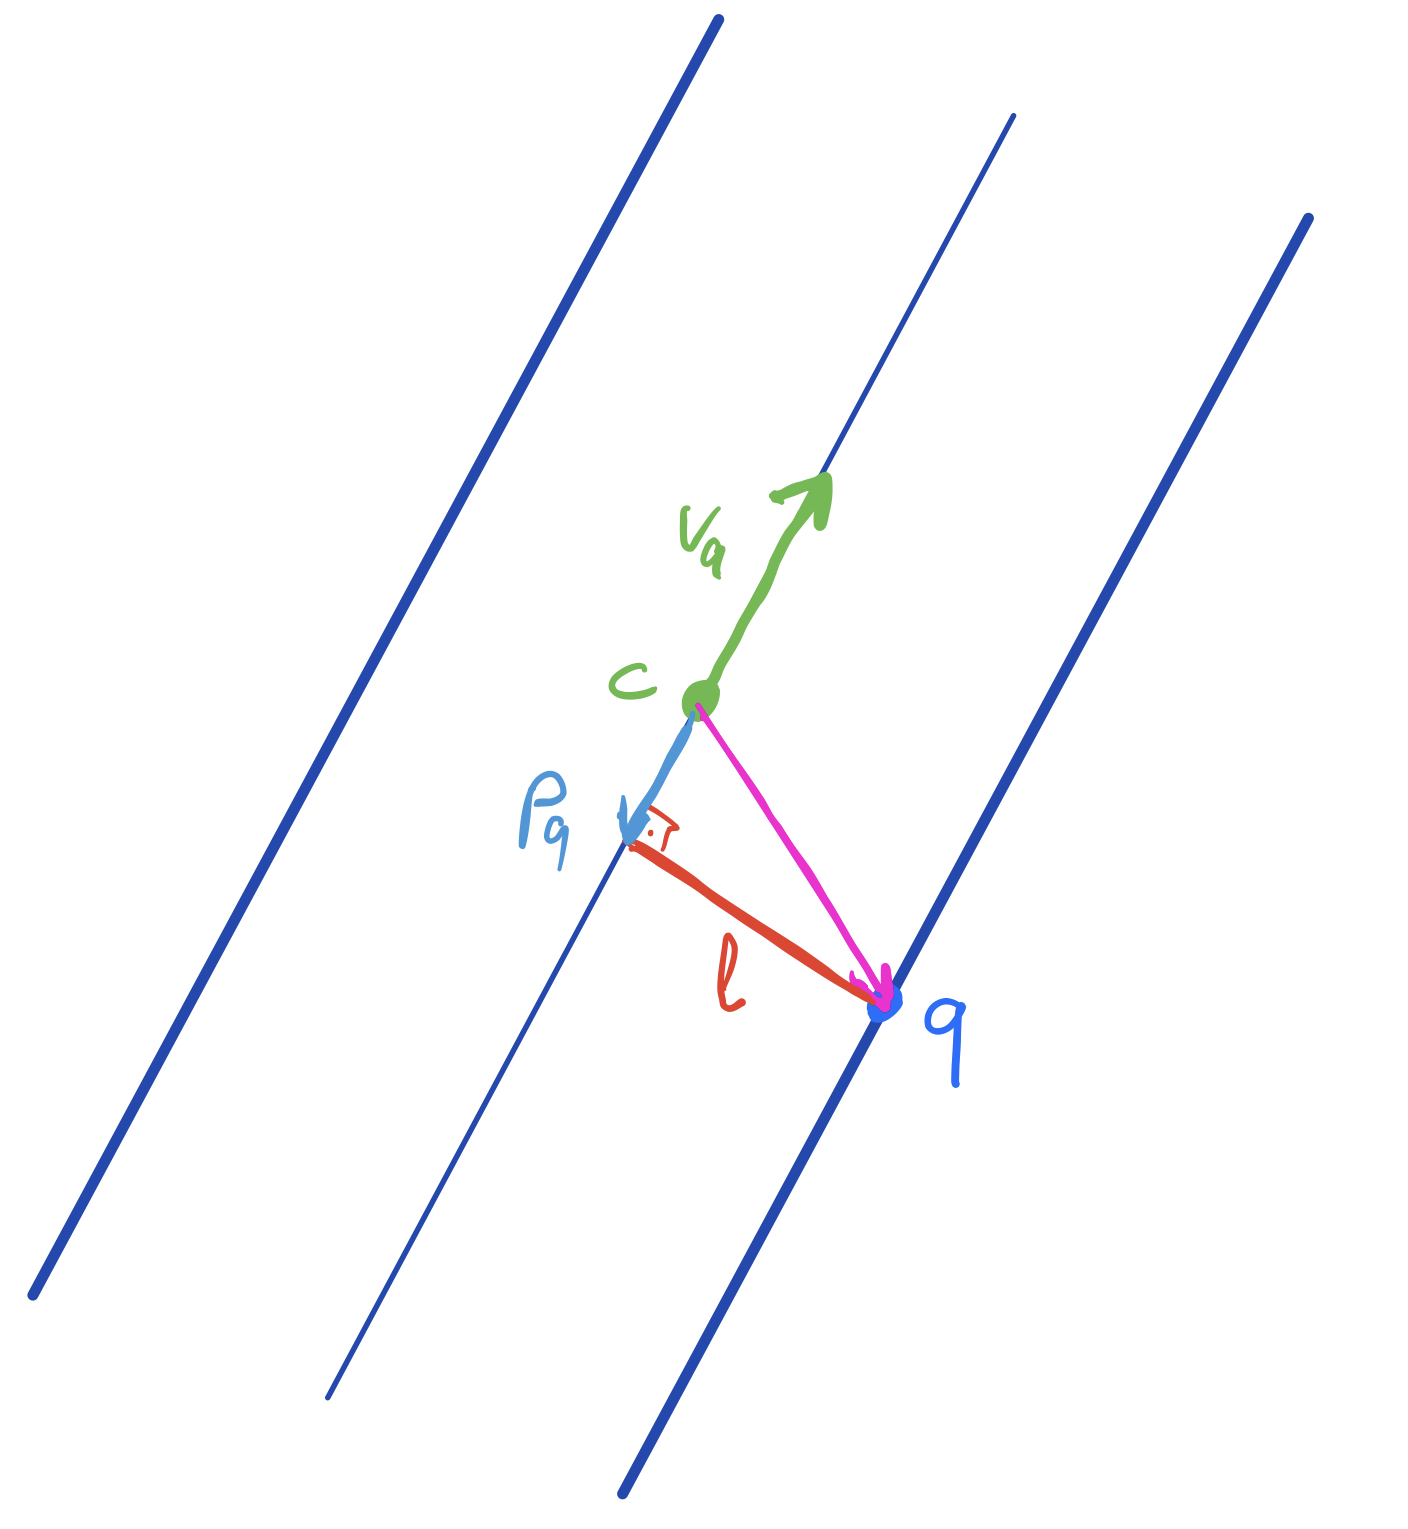
\includegraphics[width=6cm]{res/Cylinder_sketch.jpeg}
\end{figure}

We can compute $r$ as following:
First compute the orthogonal projection of the vector $c q$ on $v_a$:
$$p_q = <v_a, q-c> v_a$$
Now we can compute the vector $r$ :

\begin{gather*}
    r = q-c-p_q \\
    r = q-c - <v_a, q-c> v_a
\end{gather*}
Now we just need to compute the norm of $r$ and we have the distance we wanted. We can take this distance squared to simplify computation and we have the implicit equation for the cylinder:
\begin{gather*}
    |q-c-<v_a, q-c> v_a|^2 -r^2 = 0
\end{gather*}
for a point $q$.

Now we inject the ray parametrization as point $q$ :

\begin{gather*}
    q=p+v*t \\
    |p-c+v*t-<v_a, p-c+v*t>v_a|^2-r^2=0
\end{gather*}
We will solve this equation for $t$:
\begin{gather*}
    |p-c+v*t-<v_a, p-c+v*t>v_a|^2-r^2=0\\
    |p-c+v*t - <v_a, p-c>v_a - t*<v_a, v>v_a|^2 -r^2=0\\
    |t*(v+<v_a, v>v_a) + (p-c- <v_a, p-c>v_a)|^2 -r^2 = 0
\end{gather*}
Let us define some variables :
\begin{gather*}
    A = (v-<v_a, v>v_a)\\
    B = (p-c- <v_a, p-c>v_a)
\end{gather*}
Both are vectors.
\begin{gather*}
    |t*A + B|^2 -r^2 = 0\\
    <t*A+B, t*A+B> -r^2 = 0\\
    t^2 * <A,A> + t*<A+B, A+B> + <B,B> -r^2 = 0
\end{gather*}
We have an equation of the form:
$$t^2*C + t*E + F = 0$$
with:
\begin{align*}
    C &= <A,A> \\ 
    &= |v-<v_a, v>v_a|^2\\
    E &= 2*<A, B> \\
    &= 2*<v-<v_a, v>v_a, p-c- <v_a, p-c>v_a>\\
    F &= <B,B> -r^2 \\
    &= |p-c- <v_a, p-c>v_a|^2
\end{align*}


Now that we have these three elements, we can resolve the equation for $t$ using \textit{quadraticSolve} and keep only the smallest positive solution for $t$(to have the first intersection in front of the observer).

\section{Finite length cylinder}
Now that we have $t$ for which the ray intersect the infinitely long cylinder, we can keep only intersections that this cylinder at a distance less than $h/2$ from the center.

To do so, we compute the orthogonal projection of the vector between $c$ and the intersection point $p_i$ and check if its norm is smaller that $h/2$.

$$|<p_i-c, v_a>v_a|^2 \leq h/2$$
$$p_i = p+v*t_i$$
where $t_i$ is the solution of the last equation. We keep only intersections that satisfy this equation.


\end{document}
